%; whizzy paragraph -pdf xpdf -latex ./whizzypdfptex.sh
%; whizzy-paragraph "^\\\\begin{frame}\\|\\\\emtext"
% latex beamer presentation.
% platex, latex-beamer でコンパイルすることを想定。 

%     Tokyo Debian Meeting resources
%     Copyright (C) 2012 Junichi Uekawa
%     Copyright (C) 2012 Nobuhiro Iwamatsu

%     This program is free software; you can redistribute it and/or modify
%     it under the terms of the GNU General Public License as published by
%     the Free Software Foundation; either version 2 of the License, or
%     (at your option) any later version.

%     This program is distributed in the hope that it will be useful,
%     but WITHOUT ANY WARRANTY; without even the implied warreanty of
%     MERCHANTABILITY or FITNESS FOR A PARTICULAR PURPOSE.  See the
%     GNU General Public License for more details.

%     You should have received a copy of the GNU General Public License
%     along with this program; if not, write to the Free Software
%     Foundation, Inc., 51 Franklin St, Fifth Floor, Boston, MA  02110-1301 USA

\documentclass[cjk,dvipdfmx,12pt]{beamer}
\usetheme{Tokyo}
\usepackage{monthlypresentation}

%  preview (shell-command (concat "evince " (replace-regexp-in-string "tex$" "pdf"(buffer-file-name)) "&")) 
%  presentation (shell-command (concat "xpdf -fullscreen " (replace-regexp-in-string "tex$" "pdf"(buffer-file-name)) "&"))
%  presentation (shell-command (concat "evince " (replace-regexp-in-string "tex$" "pdf"(buffer-file-name)) "&"))

%http://www.naney.org/diki/dk/hyperref.html
%日本語EUC系環境の時
\AtBeginDvi{\special{pdf:tounicode EUC-UCS2}}
%シフトJIS系環境の時
%\AtBeginDvi{\special{pdf:tounicode 90ms-RKSJ-UCS2}}

\title{東京エリアDebian勉強会}
\subtitle{systemd}
\author{岩松 信洋\\iwamatsu@debian.org}
\date{2012年11月17日}
\logo{
\includegraphics[width=8cm]{image200607/openlogo-light.eps}}

\begin{document}

\frame{\titlepage{}}

%\begin{frame}[containsverbatim]
%
%おまえら、ちょっと 「\texttt{ps ax | grep systemd}」 実行してみろ!
%\begin{commandline}
%
%hooo%
%
%\end{commandline}
%\end{frame}

\begin{frame}{はじめに}

\begin{itemize}
\item 世の中の主要なLinuxディストリビューションは 
SysVinit の init scripts から他のinit システムに移行しつつある(はず)。
\item FedoraやArch Linuxがsystemd に移行を始めたということもあり、
一部で盛り上がっている(阿鼻叫喚ともいう)。
\item まさか いまだに SysVinit を使ってないよね?
\item Debianとsystemdについてまとめた。
\end{itemize}

\end{frame}

\begin{frame}{systemdとは?}

\begin{itemize}
\item RedHat に勤めている Lennart Poettering 氏によって開発されている。
\item init の代替プログラム。
\item 実際には init の代替だけではなく、Linux のサービス(デーモン)管理フレームワーク。
%Linux カーネル用のデバイス管理ツールである udev が systemd のソースにマージ
%されています。ログシステムもある。将来は cron や acpid などの代替え機能を
%提供する予定らしい。
\item 今までのinitシステムの違い
  \begin{itemize}
  \item サービスのプロセス管理を pid ではなく、cgroups を使う。
  \item サービスの起動をソケットとバス(dbus)を使う。
  \item サービスの依存関係があり、これによってシステム立ち上げ処理をより並列的に行える。
  \item System V スタイルとBSDスタイルの両方をサポートしている。
  \item CosoleKit との連携。
  \end{itemize}
\end{itemize}

\end{frame}


\begin{frame}
\includegraphics[width=1\hsize]{image201211/systemd-relation.eps}
\end{frame}

\begin{frame}{systemdとは?}

\begin{itemize}
\item 開発は freedesktop.orgで行われており、開発は活発で週に一度はバージョンアップ。
\item 最新バージョンは v195。
\item \url{http://cgit.freedesktop.org/systemd/systemd/}
\end{itemize}

\end{frame}

\begin{frame}{SysVinit と比べた systemd の利点}

\begin{itemize}
\item 設定が容易。
\item 起動が早い。
\item カーネルモジュールの操作、セッション管理、ログ管理、ディスクの暗号化などが統合されている。
\end{itemize}

その他、開発者による説明が\url{http://0pointer.de/blog/projects/why.html}
にある。

\end{frame}

\begin{frame}{SysVinit と比べた systemd の欠点/不安}

\begin{itemize}
\item あらゆる基本サービス(cronなども)をまとめるという壮大な物語。
\item 日本語ドキュメントがない、ぐらい?
\item kFreeBSD でも頑張ればうごくらしい。(どうやってるのかは不明)
\end{itemize}

\end{frame}

\begin{frame}{Debianで使う}

\begin{itemize}
\item systemd はもちろん Debian でも提供されている
\item testing / unstable で v44 が利用できる\\
最新版とバージョンに差があるが、アップストリームで
頻繁にバージョンアップするのでバージョンはあまり問題ではない
v44 でも systemd を十分に使うことができる

\item いまのところ Debianに関する情報は \url{http://wiki.debian.org/systemd}
にまとまっているが情報が少なく、内容も古い
\end{itemize}

\end{frame}

\begin{frame}[containsverbatim]{インストール}

\begin{itemize}
\item apt-get / aptitude でインストールできる。
\item Linux カーネルは 2.6.39 以上、devtmpfs, fanotify, autofs4, cgroups が有効になっている必要がある。
\end{itemize}

\end{frame}

\begin{frame}[containsverbatim]{インストール}

インストールは以下のように実行する。

\begin{commandline}
$ sudo apt-get install systemd
\end{commandline}
%$

以下のパッケージが依存関係でインストールされる。
\begin{commandline}
libsystemd-daemon0
libsystemd-id128-0
libsystemd-journal0
libpam-systemd
\end{commandline}
%$

\end{frame}

\begin{frame}[containsverbatim]{インストール}

\begin{itemize}
\item 次にブートローダにinit指定を追加する
\item GRUB を使っている場合、\texttt{/etc/default/grub} の
\texttt{GRUB\_CMDLINE\_LINUX\_DEFAULT} に {\bf init=/lib/systemd/systemd} を追記する
 
\begin{commandline}
変更前:
GRUB_CMDLINE_LINUX_DEFAULT="quiet"
変更後:
GRUB_CMDLINE_LINUX_DEFAULT="quiet init=/lib/systemd/systemd"
\end{commandline} 
%$

\end{itemize}

\end{frame}

\begin{frame}[containsverbatim]{インストール}

\begin{itemize}
\item 変更後、{\bf update-grub}を実行し、GRUB に設定を反映する。
\item そしてリブートする。
\item 設定が間違っていないければ systemd で立ち上がるはず。
\end{itemize}

\begin{commandline}
$ sudo update-grub
.....
$ sudo reboot 
\end{commandline}
%$

\end{frame}

\begin{frame}[containsverbatim]{起動速度}

\begin{itemize}
\item systemd はアナライザをデフォルトでサポートしている。\\
SysVinit だと bootchart2 で測定する必要がある。
\item 起動にかかった時間を確認するには \texttt{systemd-analyze} を実行する。
\begin{commandline}
$ systemd-analyze 
Startup finished in 1831ms (kernel) + \ 
     5669ms (userspace) = 7500ms
\end{commandline}
%$
\end{itemize}
\end{frame}

\begin{frame}[containsverbatim]{起動速度}

\begin{itemize}

\item また、画像で確認したい場合には \texttt{prop} オプションを指定して実行する。\\
  SVG フォーマットで出力されるので、リダイレクトしてファイルに保存する。
\begin{commandline}
$ systemd-analyze plot > systemd-boot.svg
\end{commandline}
%$
\end{itemize}

\end{frame}

\begin{frame}

\begin{center}
\includegraphics[width=1\hsize]{image201211/systemd-boot.eps}
\end{center}
\end{frame}

\begin{frame}[containsverbatim]{起動速度}

試しに自分が常用している環境で起動時間を測定したところ、
SysVinit は約15秒、systemd は約10秒だった。 

\end{frame}

\begin{frame}{用語}

systemd を扱うには専門用語が出てくるので説明する。

\end{frame}

\begin{frame}{ユニット}

\begin{itemize}
\item systemd ではデーモンなどの制御対象のことをユニットと呼ぶ。
\item ユニットにはサービス、デバイス、マウントポイントなど、いくつかの種類がある。
\item このユニットはテキストファイルで記述され、\texttt{/lib/systemd/system/} 以下に格納されている。
\item 各ユニットは拡張子を持ち、サービスの場合は\texttt{.service}となっている。
\end{itemize}

\end{frame}

\begin{frame}{ユニット}

\begin{table}[htb]
\begin{center}
  \begin{tabular}{ll}
    ユニットの種類 & 説明 \\
    service & サービス \\
    socket & ソケットで起動するためのソケット定義 \\
    target & 各サービスを同期させるための定義 \\
    device & udev で管理するデバイス \\
    snapshot & ある時点のinit の状態 \\
    timer & イベントから時間経過 \\
    path & 監視するパス \\
    mount & マウントポイント \\
    swap & スワップ \\
    automaount & 自動マウントポイント \\
  \end{tabular}
%\caption{systemd で提供するユニット}
%\label{tbl:unit}
\end{center}
\end{table}

mount, swap, automout は起動時に \texttt{/etc/fstab} から自動的に
ユニットを生成する。

\end{frame}

\begin{frame}{ターゲット}
\begin{itemize}
\item SysVinit の runlevel 相当のもの。
\item これはディストリビューションによって異なる。
\item Debianの場合は以下の通り。

\begin{table}[h]
\begin{center}
  \begin{tabular}{ll}
    run level & systemd のターゲット \\
    0 & poweroff.target \\
    1 & rescue.target \\
    2 - 5 & multi-user.target \\
    6 & reboot.target \\
  \end{tabular}
%\caption{run levelとターゲットの対応}
%\label{tbl:target}
\end{center}
\end{table}
\end{itemize}
\end{frame}

\begin{frame}{ターゲット}

\begin{itemize}
\item この他にgraphical.target と emergency.target がある。
\item graphical.target X による起動を行うときに呼ばれるターゲット
\item emergency.target は障害が起こった時に起動できるようにするためのターゲット。
\item ターゲットはカーネルのブートオプションに \texttt{systemd.unit=}で指定できる。
\item 何も指定しない場合はdefault.target が呼ばれるようになっている。
\end{itemize}

\end{frame}

\begin{frame}{ユニットの操作方法}

\begin{itemize}
\item systemd に移行した後、デーモン等の制御は /etc/init.d/ 以下を実行するのではなく、{\bf systemctl}
コマンドを使って操作する。
\item 以下にユニットの操作方法について説明する。
\end{itemize}

\end{frame}

\begin{frame}[containsverbatim]{起動しているユニットを表示する}

起動しているユニットを表示するには sytemctl を実行する。

\begin{commandline}
$ systemctl
...
console-setup.service     loaded active exited        LSB: Set console font and 
cron.service              loaded active running       LSB: Regular background pr
dbus.service              loaded active running       D-Bus System Message Bus
debian-fixup.service      loaded active exited        Various fixups to make sys
exim4.service             loaded active running       LSB: exim Mail Transport A
getty@tty1.service        loaded active running       Getty on tty1
ifup@eth0.service         loaded active exited        ifup for eth0
...
\end{commandline}
%$

\end{frame}

\begin{frame}[containsverbatim]{全てのユニットを表示する}

操作できるユニットを表示するには \texttt{--all} を指定する。
 
\begin{commandline}
$ systemctl --all
UNIT                      LOAD   ACTIVE   SUB       JOB DESCRIPTION
proc-sys...misc.automount loaded active   waiting       Arbitrary Executable Fil
dev-cdrom.device          loaded active   plugged       QEMU_DVD-ROM
dev-disk...QM00003.device loaded active   plugged       QEMU_DVD-ROM
dev-disk...QM00001.device loaded active   plugged       QEMU_HARDDISK
dev-disk...2dpart1.device loaded active   plugged       QEMU_HARDDISK
dev-disk...2dpart2.device loaded active   plugged       QEMU_HARDDISK
...
\end{commandline}
%$

\end{frame}

\begin{frame}[containsverbatim]{ユニットの状態を確認する}

ユニットの状態を確認するには、\texttt{status} オプションに確認したいユニット名を
指定して実行する。

以下に rsyslog.service ユニットの状態を確認する例を示す。
\begin{commandline}
$ systemctl status rsyslog.service
    Loaded: loaded (/lib/systemd/system/rsyslog.service; enabled)
    Active: active (running) since Wed, 14 Nov 2012 00:37:18 -0800; 22h ago
   Process: 474 ExecStartPre=/bin/systemctl stop systemd-kmsg-syslogd.service (code=exited, status=0/SUCCESS)
  Main PID: 483 (rsyslogd)
    CGroup: name=systemd:/system/rsyslog.service
           └ 483 /usr/sbin/rsyslogd -n -c5
\end{commandline}
%$

これにより、このユニットは \texttt{/lib/systemd/system/rsyslog.service}によって
\texttt{Wed, 14 Nov 2012 00:37:18 -0800}に起動していることが分かる。

\end{frame}

\begin{frame}[containsverbatim]{ユニットを起動する}

起動していないユニットを起動するには、 \texttt{start}オプションにユニット名を指定して実行する。
これは \texttt{/etc/init.d/サービス start}と同様の動きとなる。
\begin{commandline}
$ sudo systemctl start ユニット名
\end{commandline}
%$

\end{frame}

\begin{frame}[containsverbatim]{ユニットを停止する}

起動しているユニットを停止するには、\texttt{stop}オプションにユニット名を指定して実行する。
これは \texttt{/etc/init.d/サービス stop}と同様の動きとなる。
\begin{commandline}
$ sudo systemctl stop ユニット名
\end{commandline}
%$

\end{frame}

\begin{frame}[containsverbatim]{ユニットの設定を再読み込みする}

ユニットの設定を再読み込みするには、\texttt{daemon-reload}オプションにユニット名を指定して実行する。
\begin{commandline}
$ sudo systemctl daemon-reload ユニット名
\end{commandline}
%$

実際に動いているデーモンの設定、例えばhttpdの設定を再読み込みし、再起動するには \texttt{reload}オプションを使う。

\end{frame}

\begin{frame}[containsverbatim]{ユニットの自動起動を有効にする}

\begin{itemize}
\item ユニットの自動起動を有効にするには \texttt{enable} オプションにユニット名を指定して実行する。
\item 有効にすると \texttt{/etc/systemd/system/ターゲット.wants/}に\texttt{/lib/systemd/system/}にあるユニット
へのシンボリックリンクが作成される。
\item どのターゲットで自動起動が有効になるかは、ユニットファイルの \texttt{Install}セクションで指定する。
\end{itemize}

\begin{commandline}
$ sudo systemctl enable ユニット名
\end{commandline}
%$

\end{frame}

\begin{frame}[containsverbatim]{ユニットの自動起動を無効にする}

\begin{itemize}
\item ユニットの自動起動を無効にするには \texttt{disable} オプションにユニット名を指定して実行する。
\item 無効にすると、/etc/systemd/system/ターゲット.wants/にあるシンボリックリンクが削除される。
\end{itemize}
\begin{commandline}
$ sudo systemctl disabe ユニット名
\end{commandline}
%$

\end{frame}

\begin{frame}[containsverbatim]{ユニットの詳細を確認する}

\begin{itemize}
\item ユニットの詳細を確認するには \texttt{show} オプションにユニット名を指定して実行する。
\item これにより指定したユニットと他のユニット、ターゲットの関係などが分かる。
\end{itemize}

\begin{commandline}
$ sudo systemctl show rsyslog.service
Id=rsyslog.service
Names=syslog.service rsyslog.service
Requires=basic.target
Wants=syslog.socket
WantedBy=multi-user.target
Conflicts=shutdown.target
...                                                           
\end{commandline}
%$

\end{frame}

\begin{frame}[containsverbatim]{ユニットについて}

ユニットには各ユニット間の依存関係を記述することができる。
依存関係の指定として以下がある。

%\begin{table}[htb]
\begin{center}
  \begin{tabular}{ll}
    定義 & 説明 \\
    Before & そのユニットの後に起動されるべきユニット。 \\
    After & そのユニットの前に起動されるべきユニット。 \\
    Conflicts & 同時に起動できないユニット。 \\
    Service & ソケットによる起動を行うユニット。 \\
    Sockets & ソケットによるユニットの起動を行う場合のソケット情報。 \\
    Wants  & 同時に起動してほしいユニット。成功、失敗は関係ない。\\
    Requires & 同時に起動されなければならないユニット。ユニットの起動が失敗した場合は要求元も失敗する \\
    BindTo & ユニットをグループとしてまとめる。
%ユニットがなくなった場合、グループで指定されているユニットは停止される。\\
  \end{tabular}
%\caption{ユニットの依存定義}
%\label{tbl:unit-depends}
\end{center}
%\end{table}

\end{frame}

\begin{frame}[containsverbatim]{ユニットについて}

例えば、default.target の内容は以下のようになっている。

\begin{commandline}
[Unit]
Description=Graphical Interface
Requires=multi-user.target
After=multi-user.target
Conflicts=rescue.target
AllowIsolate=yes
\end{commandline}

このターゲットは
multi-user.targetと同時に起動され、multi-user.targetの後に起動する。
また、rescue.targetと同時に起動できない。

\end{frame}

\begin{frame}{まとめ}

\begin{itemize}
\item Debian でも問題なくsystemd が利用できる環境が整っている。
\item レガシーなSysVinitは捨て、新しいinitの世界へ足を踏み入れてみてはいかがでしょうか。
\end{itemize}

\end{frame}

\begin{frame}{参考文献}

\url{http://www.slideshare.net/moriwaka/systemd}

\end{frame}

\end{document}

;;; Local Variables: ***
;;; outline-regexp: "\\([ 	]*\\\\\\(documentstyle\\|documentclass\\|emtext\\|section\\|begin{frame}\\)\\*?[ 	]*[[{]\\|[]+\\)" ***
;;; End: ***
